\chapter*{Введение}
\addcontentsline{toc}{chapter}{Введение}

%(Тема: Упрощение текстов на русском языке)

%\textbf{\textit{•	обоснование выбора темы, определяемого ее актуальностью}}\\

Упрощение текста, в узком смысле, -- это процесс понижения лингвистической сложности текста при сохранении исходной информации и смысла. В более широком смысле это понятие охватывает и другие операции: концептуальное упрощение содержания и формы текста; уточнение для подчеркивания ключевых моментов; обобщение для исключения второстепенной или не относящейся к теме информации ~\cite{sikka_survey_2020}.

В последние десятилетия количество неструктурированных текстовых данных резко возросло в связи с появлением Интернета. Как следствие, возросла и потребность в их упрощении, что показано на рисунке \ref{fig:growth_of_interest}. 

\begin{figure}[h!]
	
	\centering{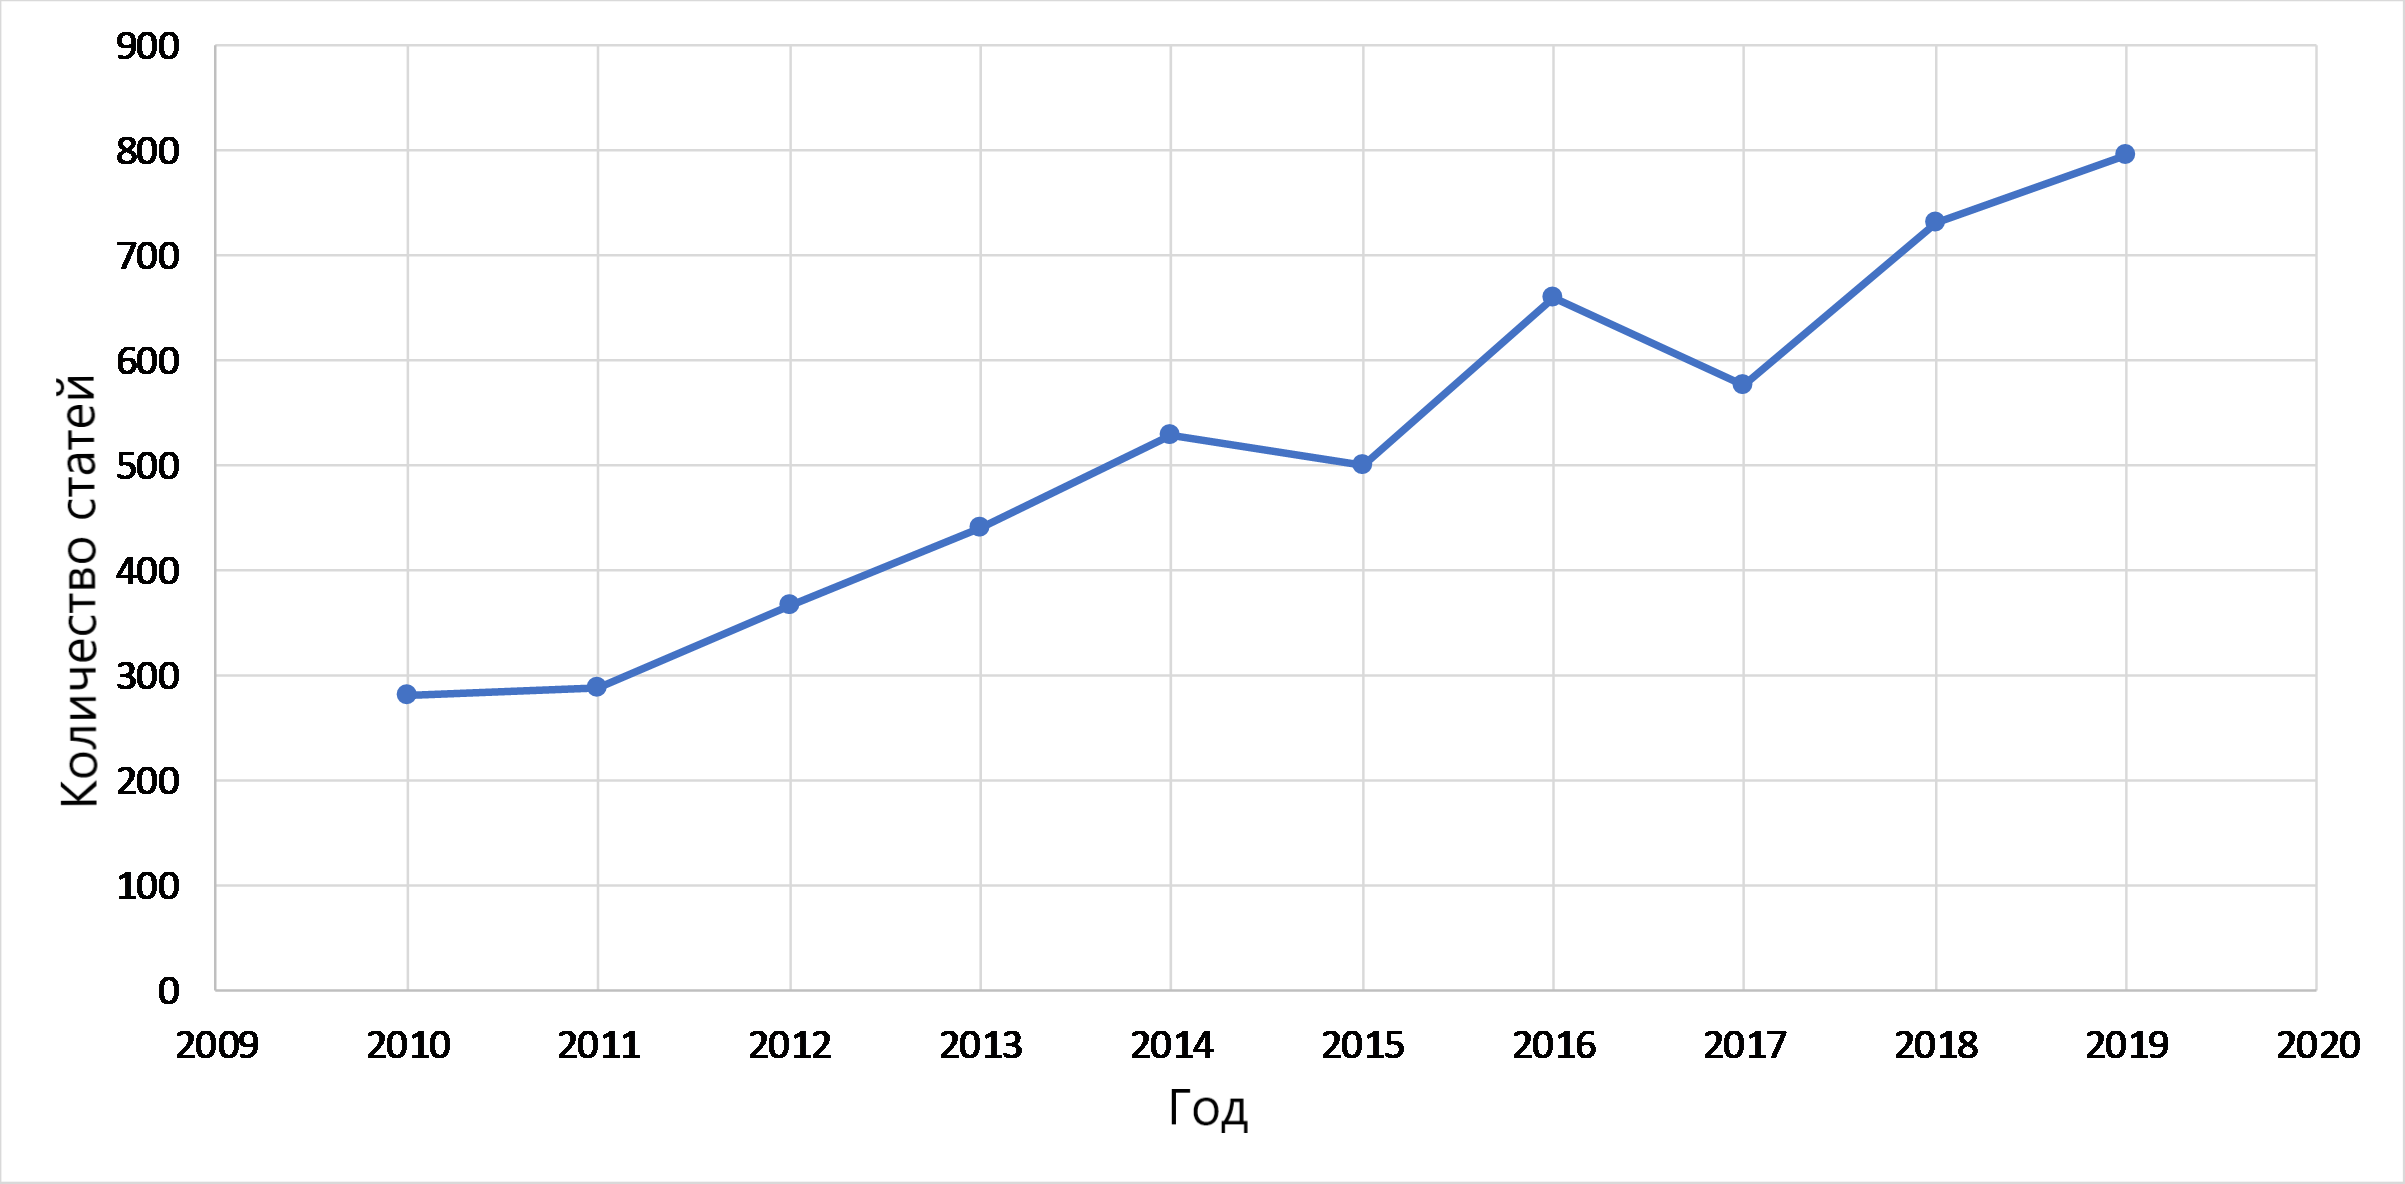
\includegraphics[scale=0.25]{inc/img/growth_of_interest.png}}
	
	\caption{График роста интереса к теме упрощения текста. Создано на основе статистики Google Scholar по поисковым запросам "Text Simplification" ("Упрощениие текстов"),  "Lexical Simplification" ("Лексическое упрощение"), "Syntactic Simplification" ("Синтаксическое упрощение")}
	
	\label{fig:growth_of_interest}
	
\end{figure}

Упрощение текстов необходимо для различных задач и целевых аудиторий: 
\begin{itemize}
	\item в качестве этапа подготовки текста перед его обобщением ~\cite{finegan_dollak_sentence_2016}; 
	\item для людей, изучающих иностранный язык, и детей, учащихся читать (требуется лексическое упрощение для сокращения количества специализированных и нечастотных слов) ~\cite{liu_simplification_2016};
	\item для людей с дислексией и афазией, для которых особенно длинные слова и предложения могут представлять трудности;
	\item для людей, страдающих аутизмом (необходимо уменьшать количество образных выражений и синтаксическую сложность) ~\cite{evans_evaluation_2014}.
\end{itemize}

%\textbf{\textit{проблема и круг вопросов, необходимых для ее решения}}\\

Упрощение предложений привлекло многих исследователей в связи с появлением больших параллельных корпусов. Наиболее известные из них - PWKP и Wiki-large. Последний представляет собой большой параллельный корпус на английском языке, состоящий из сложных предложений, взятых из Википедии, и их выровненных упрощенных версий. 

Одна из причин, по которой упрощение текстов еще не начали активно применять в приложениях на русском языке, заключается в том, что наиболее значительные общедоступные наборы данных принадлежат английскому домену, тогда как качество моделей сильно зависит от объема и количества тренировочных данных. Более того, во многих решениях имеет место фокусировка на текстах Википедии, что ограничивает исследования и приводит к неадекватности моделей на других типах данных ~\cite{kazan_federal_university}. 

Другая тема для обсуждения -- выбор уровня, на котором текст будет упрощаться. В целом, упрощение текста подразумевает изменения на разных уровнях, включая стилистический, грамматический и лексический уровни. На данный момент одним из наиболее популярных подходов является упрощение текста <<предложение за предложением>> ~\cite{galeev_rubts_2021}. (!!Этот подход к какому из названных Вами уровней относится?) В нем в качестве подзадачи применяются перефразирование и генерация текста на естественном языке.

\textbf{\textit{•	объект исследования или разработки, цель работы с ее разделением на взаимосвязанный комплекс задач, подлежащих решению}}\\


Объектом исследования данной работы является общая задача упрощения текстов на русском языке на уровне предложений. Цель -- разработка качественной модели, решающей эту проблему.

В рамках выполнения работы необходимо решить следующие задачи: 
\begin{enumerate}[label={\arabic*)}]
	\item собрать или найти крупный параллельный корпус на русском языке, состоящий из сложных предложений и их выровненных упрощенных версий и основанный на разных типах источников;
	\item подобрать метрики, по которым можно определить качество упрощения;
	\item изучить существующие подходы к решению задачи упрощения текстов на уровне предложений как на русском, так и на иностранных языках;
	\item разработать или адаптировать к русскому языку несколько моделей, решающих эту задачу;
	\item провести сравнительный анализ разработанных моделей, обученных как на всем собранном корпусе, так и на его отдельных частях (основанных на разных типах источников);
	\item выбрать наилучшую модель.
\end{enumerate}


%\textbf{\textit{•	методы исследования}}\\


Упрощение предложений можно рассматривать как задачу <<от последовательности к последовательности>> (sequence-to-sequence, seq2seq)~\cite{kazan_federal_university}, к которой применимы нейронные модели языка. Такая модель получает на вход исходное предложение, а на выходе выдает его упрощенную версию.

(!В статье "A Survey on Text Simplification" выделяется множество подходов. Почему Вы вынесли сюда именно его? Детально анализировать все подходы нужно будет, конечно, не во Введении, а в Аналитическом разделе ВКР (ну или, я так понимаю, в Вашем случае - в самой НИР), но во Введении нужно хотя бы рассказать, как вообще современное научное сообщество понимает "упрощение" текста и кратко, обобщённо пересказать общую суть разных групп подходов к этой задаче.)

Поняте <<простота тектса>> имеет субъективную природу (особенно при упрощении предложений с помощью моделей seq2seq), поэтому наилучшим образом оценить качество результата может только человек, проанализировав полученное упрощенное предложение с точки зрения грамматики, сохранения смысла и простоты. Однако такая оценка слишком долгая и трудоемкая, поэтому был разработан ряд специальных метрик, из которых SARI на данный момент признана наиболее удачной ~\cite{xu_optimizing_2016}. 

(!Опять же, я думаю, стоит обобщить существующие метрики, разделить их на какие-то категории, если у них есть что-то общее, и очень-очень кратко перечислить, на чём в принципе основывается та или иная группа метрик, с указанием примеров конкретных метрик.)


\textbf{\textit{•	краткий обзор базы исследования и литературных источников}}\\



Задача упрощения текстов на русском языке была предложена в рамках международной конференции по компьютерной лингвистике и интеллектуальным технологиям DIALOGUE 2021 \footnote{\url{http://www.dialog-21.ru/dialogue2021/results/}}. Организаторы подготовили обучающие и тестовые наборы с использованием краудсорсинговой платформы, а также перевели тексты из Википедии (корпус RuWikiSimple). Другим источником данных могут стать результаты перевода в виде перефразирования~\cite{kazan_federal_university}. 

(!Впервые? Или почему Вы именно эту конференцию во Введение вынесли?)

В последнее время достигнуты хорошие результаты в решении проблемы упрощения предложений. Модель-трансформер mBART, первоначально разработанная для машинного перевода, оказалась эффективной для решения задач такого рода, в особенности при добавлении специальных маркеров управления ~\cite{martin_muss_2021}.

В основе большинства современных моделей лежит подход encoder-decoder (кодировщика-декодера), зачастую дополненный и другими инструментами. Например, модель DRESS ~\cite{fang_learning_2017} добавляет в архитектуру encoder-decoder подход обучения с подкреплением: выполняется обзор возможных упрощений и выбирается наилучший из них.
 
  Решение, победившее в соревновании, организованном в рамках конференции DIALOGUE 2021,  в значительной степени основано на системе MUSS (Multilingual Unsupervised Sentence Simplification, система мультиязычного упрощения, обучающаяся без учителя) ~\cite{martin_muss_2021}. Модель состоит из mBART, настроенного на корпусах ParaPhraserPlus\footnote{\url{https://metatext.io/datasets/paraphraser-plus}} (пары предложений на русском языке, разделенные на 3 класса по степени "перефразированности") и RuWikiSimple, в которую добалены управляющие токены (расстояние Левенштейна, доля совпадающих символов между оригинальным и упрощенным предложениями, сходство лексем).
 
 Модели, занявшие следующие места - генеративные модели на основе GPT, настроенные на отфильтрованном корпусе RuWikiSimple.
 
 (!Не хватает какого-то завершения Введения. Например, в статье "Система автоматического аннотирования текстов с
 помощью стохастической модели" Введение заканчивается словами:
 "Таким образом, на сегодняшний день оценка качества аннотирования не обходится без
 работы экспертов, что безусловно дорого и требует существенных временных затрат."
 
 Надо как-то подвести итог, в каком состоянии находится сейчас решаемая задача и обозначить место Вашей работы в текущем положении вещей.)

~\cite{martin_muss_2021}
\cite{voznesenskaya_automatic_2018}
~\cite{kazan_federal_university_kazan_russia_rusimplesenteval-2021_2021}
~\cite{noauthor_bart_nodate}
~\cite{noauthor_191013461_nodate}
~\cite{saint_petersburg_russia_rusimscore_2021}






